\documentclass{article}

% Language setting
% Replace `english' with e.g. `spanish' to change the document language


% Set page size and margins
% Replace `letterpaper' with `a4paper' for UK/EU standard size
\usepackage{geometry}
 \geometry{
 a4paper,
 total={170mm,257mm},
 left=20mm,
 top=20mm,
 }
%Packages
%Coloums

%\usepackage{tabularx}
%\usepackage{amsmath}
\usepackage{graphicx}
\usepackage[colorlinks=true, allcolors=blue]{hyperref}
\usepackage{titlesec}
\usepackage[square,numbers]{natbib}

\graphicspath{ {../images/} }
\bibliographystyle{abbrvnat}

\title{Project Life Cycles}
\author{Chris Hadden}

\begin{document}

\maketitle

\tableofcontents

\section{(P1) The different phases in a project life cycle}
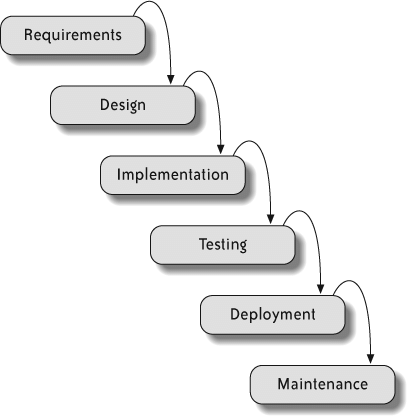
\includegraphics[scale=0.5]{Modern-Waterfall-Diagram}
\cite{modernwaterfall}
\subsection{Initiation phase}
The initiation phase is where we setup and define what the project is gonna be and who should produce this project. This will normally start with a business case or a project charter.
Before we start a project we have to decide if the project is a "go" or green. This is done by the important stakeholders who will help decide.
Finally we need to work out who the client or target audience is.
It will be important to create a Project Initialtion Document with provides the purpose for the project.\cite{kiss}

This phase in the project is equivalent to in waterfall is: Requirements

\subsection{Planning phase}
The planning phase is when we set the scope of the project. This will be the reference document used by the project manager.
If you have failed to planned then you are planning to fail.
This plan will include the cost, quality and timescale of the project, it might also show what resources are available.

Two popular ways to define goals are to use SMART and CLEAR 

SMART means
\begin{itemize}
    \item Specific Set exact goals and be specific and bounded as possible
    \item Measurable We need to set goals we can measure so we know when we did them
    \item Attainable It has to be possible to do the goals
    \item Realistic We need to be able to hit the goal with our resources
    \item Timely We have to set how long it will take
\end{itemize}

  
CLEAR means 
\begin{itemize}
    \item Collaborative Work together to hit goal
    \item Limited Have a limited scope
    \item Emotional Should engage people
    \item Appreciable Break down big goals
    \item Refineable Refine goals as we progress
\end{itemize}

This phase in the project is equivalent to in waterfall is: Design

\subsection{Execution phase}
The execution phase the team are going to develop the product. 
This phase begins with a inital meet with a the client, this will be met with an a set of reports and updates. 

What is done in the the execution phase are:
\begin{itemize}
    \item Project introduction - Everyone says hello 
    \item Develop team - Mix peoples skills
    \item Execute project management plans
    \item Set up tracking systems - Could be on paper or spreadsheet
    \item Task assignments are executed - So people have work
    \item Status meetings
    \item Update project schedule - We need to know when goals are hit
    \item Modify project plans as needed when things change
\end{itemize}

This phase in the project is equivalent to in waterfall is: Implementation/Deployment

\subsection{Project Monitoring}
Project performance monotoring means that we will know the the results of the project match up with the goals and plan.
Project managers set up Key Performance Indictators (PKI) that let us know if the project is on track.

Most common KPIs are
\begin{itemize}
    \item Project Objectives - Are we on schedule
    \item Quality Deliverables - Are tasks met
    \item Effort and Coset Tracking - Good to know if a completion data will be hit
    \item Project Performance - Monitors changes in project.
\end{itemize}

\subsection{Finishing phase}

Once a project is completed the team will have to close it. Project managers will hold a meeting after the project has officially ended to evaluate what made the project become so successfully or what where the pit falls that causes the project to fail.

There are still task for the project manager to do after the project has officially closed.The project manager will have to create a project punch, this will create a list of points that didn't get accomplished during the life time of the project and to work with the team to complete them. Create a final project report and final project budget. Finally, they will need to collect all project deliverables and  documents and store them in a single place.

This phase in the project is equivalent to in waterfall is: Maintenance

\break
\section{(D1) The importance of each development phase of the identified project life cycle}

\subsection{Initiation Phase}
The initiation phase is important as it bootstraps our abstract ideas into a meaningful goal. This stage will develop a model and define how the project will be made but to do this we need to determine the need for the project.

This phase is important esepcially in the likes for Waterfall as this is the foundation of the project. If this is wrong then the rest of the project will be wrong.
There will be a need to have highly skilled project managers in charge as stake holders to make sure that they can decide if they have enough information and research to say if the project can continue.
Also they need to be skillful to be able to make the Project Initiation Document.

A case in point is Sainsbury's warehouse automation. They did an inital roll out that has horrendous issues, they ignored that information and carried on. Two years later they had to scrap the whole project which cost one hundred and fifty million pounds. \cite{Sainsbury}



\subsection{Planning phase}
During the planing phase we to pay a lot of attention so that we all understand how this project will be made and what is need to it be done. One of the easy ways to getting goals in S.M.A.R.T. This method ensures that the goals have been thoroughly thought thought and it also provides a clear understand of what is to be done. \\

Spotify is a well know music streaming service which has used the Agile practices. They use this so that they can release new features continuously.
This impacts their planning as it means that they use "Squads", small cross functional teams to make deliveries. Every few weeks they plan and work on new things to get delivered. This allows them to adapt to user and market demands. \cite{spotify} This is seen as a very sucessful model that many other companies now use.


\subsection{Execution phase}
The execution phase is the part where the team release the product. The responsibilities of the project manager will expand, this means that you have to be able to establish an efficient workflow and carefully monitor the progress of your team. 

Another responsibility that the project manager will have during this phase as well, is to consistently maintain collaboration between the project stakeholders. We have to do this because if we didn't then their wouldn't be the improve efficiency and increased productivity that we want in the project. This can be hard to do as it can be hard to get different stakeholders to collaborate.

One of if not the most successful IT companies ever is Apple, but they have not managed to get where they are with out some disasters. Apple was in competition with Microsoft with they had launched Windows 95. At that time Apple were developing System 8 as their competition. Various project managers in Apple did not think about how to execute their project sucesfully and instead they let feature creep come in, which is where new goals and requirements are added with out any planning being put in place. This made their product become unstable and did not impress anyone. \cite{Sainsbury}

\subsection{Finishing phase}

Once a project is complete, the team must formally close it. Project managers generally hold a post mortem meeting to evaluate successes and failures. Project close helps a team identify things that went well and areas for improvement.

Famously one project that created a product but failed after release was Sony's Betabax \cite{betamax}. Sony not only had a better product than JVC's VHS tapes, but they got to market earlier as well. The reaspn Betamax failed was the Sony though they had suceeded once they went to market. Had they done a post mortem they could have found they were not competitive.

Once the project is complete, PMs still have a few tasks to complete before it is officially closed. They will need to create a project punchlist of things that didn’t get accomplished during the project and work with team members to complete them. Perform a final project budget and prepare a final project report. Finally, they will need to collect all project deliverables and  documents and store them in a single place. 

When a project is finished, the group needs to end it. Project managers will convene a post mortem meeting to assess what factors contributed to the project's success or identify potential failure points.

Even after the project is formally concluded, the project manager still has tasks to do.The project manager will need to draft a project punch, which will compile a list of tasks that were left undone over the project's duration and assign the team members to do them.Compile the project's final budget and report.Lastly, they must gather and keep all project deliverables and documentation in one location.    

It could be tempting for project managers to not do this phase as it takes time and takes people away from working on exciting new features. However not doing this phase as Sony saw could mean that important work is not done or it could mean complete failure.

\break
\bibliography{bibliography}


\end{document}
